
\chapter{Developer documentation}

\section{Specification}

\section{Algorithms and data structures used}

\subsection*{The represation of a metaprogram}

C++ template metaprogramming can be seen as a form of purely functional
programming. TODOCITE In functional programming a program's main components
are the functions. In metaprogramming, functions are represented by so called
metafunctions. Metafunctions are basically templated structs or classes, which
get their parameters as template parameters, and return values by defining
member types or compile time constants based on the template parameters.

For a specific metaprogram, Metadebugger represents only the metaprogram's call
graph. For example instantiating int_<fib<5>::value> would be represented by
the following graph in Metadebugger:

\includegraphics[width=0.3\textwidth]{img/fib5_call_graph.eps}

\subsection*{Forwardtrace}

\subsection*{Stepping}

\subsection*{Command matching}

\section{Class hierarchy}

%UML stuff
%automaton

\section{Libraries used}

\subsection*{Boost\cite{boost}}

Boost is a set of open source C++ libraries that provide ready to use solutions
to common tasks. In Metadebugger several Boost libraries are being used:
\begin{description}
    \item[Boost.Graph] \hfill \\
        This library provides a generic interface and implementations of graph
        data-structures and algorithms.

        In Metadebugger the information which is gathered by Templight is
        stored in a Boost.Graph data-structure. Since the whole program is
        revolving around the metaprogram which being debugged, it was very
        important to choose a robust and flexible graph library.
    \item[Boost.Optional] \hfill \\
        Unlike in some programming languages, in C++ stack allocated objects
        cannot have a null value. This have some advantages, for example the
        programmer doesn't have to check for a null value before doing
        operations on an object.

        But at the same time, sometimes it is useful to have an object state,
        in which the object is invalid in purpose. Boost.Optional provides an
        easy way to turn any type into a type which can have an invalid state
        called \lstinline|boost::none|.
    \item[Boost.PropertyTree] \hfill \\
        The Boost.PropertyTree library provides a data structure that stores an
        arbitrarily deeply nested tree of values, indexed at each level by some
        key.

        Metadebugger makes use of the xml parsing capabilites of
        Boost.PropertyTree to parse the xml created by Templight.
    \item[Boost.Filesystem] \hfill \\
        Boost.Filesystem provides cross platform solutions to manipulate the
        file system.

        Metadebugger uses Boost.Filesystem to create and delete the temporary
        file where the output of Templight is stored until it's processed.
    \item[Boost.StringAlgorithm] \hfill \\
        Boost.StringAlgorithm provides a handful of useful string-related
        algorithms.

        Metadebugger has to manipulate strings in various contexts and makes
        use of a few algorithms contained in this library.
    \item[Boost.LexicalCast] \hfill \\
        Boost.LexicalCast provides an easy way to convert numbers to string
        form and the other way around.

        Metadebugger uses this library during parsing of the Templight xml
        file.
\end{description}

\subsection*{Just\cite{just}}

Just is a collection of lightweight C++ libraries. The following Just libraries
are used in Metadebugger:
\begin{description}
    \item[just::console] \hfill \\
        The just::console library provides a cross platform interface to output
        colored text to a console interface.

        Metadebugger uses colored text in its output for easier readability.
    \item[just::test] \hfill \\
        Just::test is a testing library.

        Metadebugger uses just::test to create unit and integration test cases.
\end{description}

\subsection*{Clang\cite{clang}}

Clang is a C++ frontend for LLVM. Together they form a highly customizable C++
compiler. Clang is used to compile the source code given as an input to
Metadebugger.

\subsection*{Templight\cite{templight}}

Templight (in its current form) is a source code patch to Clang. With
Templight, Clang is able to generate output about the template instantiation
steps during compilation. Metadebugger takes this output and creates the
necesseary data structures to be able to simulate the compilation.

\subsection*{Readline\cite{readline}}

The Readline library is the de facto standard library used to handle user
inputs in software that uses an interactive command line interface.

\section{Architecture}

\section{Testing}

\subsection{Test plan}

\subsection{Unit tests}

\subsection{Integration tests}

\section{Possible further improvements}

%A Fejlesztõi dokumentáció tartlmazza
%\begin{itemize}
%\item a probléma részletes specifikációját,
%\item a felhasznált módszerek részletes leírását, a használt fogalmak definícióját,
%\item a program logikai és fizikai szerkezetének leírásár (adatszerkezetek, adatbázisok, modulfelbontás),
%\item a tesztelési tervet és a tesztelés eredményeit.
%\end{itemize}
